\documentclass[a4paper, 10pt]{article}
\usepackage[spanish] {babel}
\title{Trabajo Practico 3}
\usepackage{floatflt}
\usepackage{tpalgo3}
\usepackage{caratula}
\usepackage[pdftex]{graphicx}
\usepackage{color}

\setlength{\leftmargin}{2cm}
\setlength{\rightmargin}{2cm}
\setlength{\oddsidemargin}{-1cm}
\setlength{\evensidemargin}{-1cm}
\setlength{\topmargin}{-1cm}
\setlength{\textwidth}{18cm}
\setlength{\textheight}{25cm}

\usepackage{fancyhdr}
\pagestyle{fancy}
\fancyhf{}
\fancyhead [LO,LE]{\scriptsize Trabajo Pr\'actico N$^{\circ}$3 - Reentrega}
\fancyhead [RO,RE]{\scriptsize Blandini, Mancuso, Mataloni, Villaverde}
\fancyfoot[CE,CO]{\thepage}
\renewcommand{\footrulewidth}{0.4pt}

\usepackage[pdftex, bookmarks=true, colorlinks, citecolor=black, linkcolor=black]{hyperref}
\usepackage{multirow}

\begin{document}

\materia{Algoritmos y Estructuras de Datos III}
\submateria{Primer Cuatrimestre de 2009}
\titulo{Trabajo Practico N$^{\circ}$3 \\ \vspace*{0.5em} Reentrega}
\grupo{Grupo 10}
\integrante{Mancuso Emiliano}{597/07}{emiliano.mancuso@gmail.com}
\integrante{Villaverde Bacskay Romina}{740/07}{romina.villaverde@gmail.com}
\integrante{Mataloni Alejandro}{706/07}{amataloni@gmail.com}
\integrante{Blandini Juan}{509/07}{juanboca@gmail.com}
\maketitle
\newpage

\addcontentsline{toc}{section}{\'Indice}
\tableofcontents


\newpage
%\fancyhead [CE,CO]{\scriptsize -\thesection -}
\begin{large}\textbf{Conjunto Independiente de Peso M\'aximo}\end{large} \\

Sea $G=(V,E)$ un grafo. Cada v\'ertice $v \in V(G)$ tiene asociado un peso positivo $p(v)$. Un subconjunto de v\'ertices $V' \subseteq V(G)$ es un conjunto independiente si los v\'ertices no son adyacentes 2 a 2. El peso de un conjunto independiente, $p(V')$, se define como la suma de los pesos de cada v\'ertice de $V'$, es decir, $p(V')=\sum_{v \in V'} p(v)$.

El problema del CONJUNTO INDEPENDIENTE DE PESO M\'AXIMO (CIPM) consiste en encontrar el subconjunto de v\'ertices independiente, cuyo peso sea m\'aximo.
\section{Ejemplos de la Vida Real}
\begin{itemize}
\item Describir situaciones de la vida real que puedan modelarse utilizando CIMP.
\end{itemize}
En un \'area alejada de Capital Federal, se encuentran ubicados muchos restaurantes de paso que pertenecen al se\~{n}or Gonz\'alez.

Pero como en este \'ultimo tiempo se le est\'a complicando administrar los restaurantes, decide cerrar algunos de ellos.
Decide mantener abiertos los locales que mejor ganancia dejen y se encuentren a m\'as de 500 metros de cualquiera de sus otros restaurantes, para no perder clientes.

Esta situaci\'on puede modelarse utilizando CIMP, ya que podemos considerar que cada nodo represanta un restaurant, cuya ganancia ser\'ia el peso del nodo; y dos nodos son adyacentes si los restaurantes que representan se encuentran a menos de 500 metros de distancia. \\

Otra situaci\'on que podemos modelar utilizando CIMP es la siguiente. En un colegio secundario se realizan distintas actividades: arte, teatro, canto, m\'usica, diversos deportes y m\'as, donde cada alumno puede realizar m\'as de una actividad. Las autoridades del colegio quieren elegir un equipo de delegados entre todos los alumnos de manera tal que dentro de una actividad no haya m\'as de un delegado, lo que es an\'alogo a que no hayan dos alumnos que sean delegados y que adem\'as realicen la misma actividad.

Tambi\'en se quiere que los alumnos que sean elegidos como delegados tengan el mayor promedio posible.

Para modelar esta situaci\'on utilizando CIMP, podemos representar a los alumnos con los nodos, donde su peso representa el promedio del alumno; y dos nodos son adyacentes si los alumnos que \'estos representan realizan una actividad juntos.

\section{Estructuras Utilizadas}
Para representar el grafo utilizamos una lista de adyacencia. Adem\'as, contamos con otras estructuras que describiremos a continuaci\'on, para facilitar la implementaci\'on del algoritmo y las heur\'isticas.

\subsection{Clase \texttt{Vertice}}
Esta clase la utilizamos para representar un nodo. Sus atributos son:
\begin{itemize}
\item \texttt{numero}: de tipo \texttt{int} que representa el n\'umero del nodo.
\item \texttt{peso}: de tipo \texttt{int} que representa el peso del nodo.
\item \texttt{vecinos}: \texttt{ArrayList<Vertice>}. Esta lista contiene todos los vecinos del nodo ordenados por su n\'umero.
\item \texttt{componenteConexa}: de tipo \texttt{int} que representa el n\'umero de componente conexa a la que pertenece.
\end{itemize}

\subsection{Clase \texttt{Soluci\'on}}
Con esta clase representamos tanto las soluciones parciales que se van generando durante la ejecuci\'on del algoritmo y las heur\'isticas, y tambi\'en la soluci\'on final, de cada componente conexa y del grafo. Sus atributos son:
\begin{itemize}
\item \texttt{conjunto}: \texttt{ArrayList<Vertice>}. Representa al conjunto de v\'ertices que forman parte de la soluci\'on, por lo tanto, no son adyacentes dos a dos.

\item \texttt{posibles}: \texttt{ArrayList<Vertice>}. Representa a los posibles v\'ertices para agregar al conjunto, \'estos son aqu\'ellos que no tienen ning\'un vecino que forme parte de \'esta. Esta lista la actualizamos cada vez que agregamos y sacamos un nodo de la soluci\'on parcial.

\item \texttt{adyacencias}: \texttt{int[]}. Contador de veces que cada nodo es adyacente a alguno de la soluci\'on, es decir, la posici\'on $i$ del array indica cu\'antos vecinos tiene el v\'ertice $i$ en la soluci\'on parcial. Este array los actualizamos cada vez que agregamos un nodo a la soluci\'on y cada vez que eliminamos uno para encontrar otra soluci\'on mejor.

\item \texttt{peso}: de tipo \texttt{int} que representa el peso total del conjunto de nodos que forman parte de la soluci\'on.

\item \texttt{sacarDeSolucion}: este m\'etodo toma como par\'ametro un v\'ertice para sacar de la soluci\'on. Lo elimina del conjunto de v\'ertices, actualiza el peso de la soluci\'on y actualiza el arreglo de adyacencias indicando que los vecinos de este v\'ertice tienen un adyacente menos en la soluci\'on, y si para cada uno de estos v\'ertices, no qued\'o ning\'un vecino en la soluci\'on, lo agrego a la lista \texttt{posibles}, para que sea considerado en las pr\'oximas iteraciones.

\item \texttt{agregarASolucion}: este m\'etodo toma como par\'ametro un v\'ertice para agregar a la soluci\'on. Agrega el v\'ertice al conjunto, actualiza el peso de la soluci\'on y actualiza el arreglo \texttt{adyacencias} incrementando en 1 la cantidad de adyacentes que tiene cada uno de sus vecinos en la soluci\'on.
\end{itemize}

\subsection{Inicializaci\'on de la Estructura de Datos}
\begin{itemize}
\item Como la primera l\'inea del archivo representa la cantidad de nodos del grafo, creamos los v\'ertices que necesitamos.
\item En cada l\'inea que leemos tenemos la informaci\'on del nodo. Por lo tanto, cada vez que leemos una l\'inea, asignamos los atributos del v\'ertice: su n\'umero, su peso y sus vecinos.
\item Llenamos la lista \textit{vertices} que contiene los v\'ertices del grafo. S\'olo para la heur\'istica constructiva la ordenamos de forma descendente seg\'un su peso utilizando \textit{QuickSort}, ya que en cada iteraci\'on agregamos el v\'ertice de mayor peso, siempre que sea posible.
\end{itemize}

\subsection{Aclaraci\'on sobre el c\'alculo de las complejidades}
Para calcular la complejidad de los algoritmos, usamos el modelo uniforme, puesto que podemos considerar los pesos de los nodos acotados por un cierto n\'umero (el peso m\'aximo), y por lo tanto las operaciones b\'asicas, como agregar un nodo a una soluci\'on parcial, sumar y restar un entero que representa al peso, etc, las consideramos como constantes; es decir, la complejidad del algoritmo no depende de los pesos que tengan los nodos, sino del tama\~no del grafo (la cantidad de nodos y aristas).

\newpage

\section{Algoritmo Exacto}
Desarrollar e implementar un algortimo exacto para CIPM.

\subsection{Introducci\'on}
Como ten\'iamos que desarrollar un algoritmo exacto para resolver el problema, s\'i o s\'i tenemos que evaluar todos los casos que potencialmente pueden ser una soluci\'on y quedarnos con el conjunto de nodos, tales que no sean adyacentes dos a dos y adem\'as, que el peso sea m\'aximo. Como estamos buscando obtener un conjunto independiente de peso m\'aximo, separamos el grafo en componentes conexas utilizando BFS, aplicamos el algoritmo exacto para cada una de ellas, y luego unimos las soluciones de cada una. Esto lo podemos hacer ya que entre cada componente conexa los nodos no se comunican entre s\'i; por lo tanto el conjunto que nos queda al unir la soluci\'on de cada una de las componentes conexas es independiente. \\

Para cada componente conexa debemos calcular el subconjunto independiente de peso m\'aximo. Para ello debemos evaluar todos los posibles subconjuntos que puedan llegar a formar parte de la soluci\'on del grafo de manera ordenada, y quedarnos con el de mayor peso. Por esto es que decidimos implementar un algoritmo que utilice la t\'ecnica de $backtracking$ para resolver el problema.

\subsection{Descripci\'on y Correctitud de los Algoritmos}

Para resolver este problema utilizaremos las siguientes estructuras:
\begin{itemize}
	\item La lista de los v\'ertices $vertices$, en la cual est\'an los v\'ertices de la componente conexa; 
	\item Un array de enteros $adyacencia$, en el cual en la posici\'on $i$ me va a indicar cu\'antos v\'ertices de la soluci\'on son adyacentes al v\'ertice $v_i$; 
	\item Una pila $indices$, que en cada iteraci\'on, se apila la posici\'on del nodo que se acaba de agregar a la soluci\'on;
	\item Un entero $peso$, que indica el peso total del subconjunto de nodos de la soluci\'on; 
	\item Una lista $solucionComponenteConexa$ donde se guarda la mejor soluci\'on de esa componente conexa;
	\item Una lista $solucionParcial$ que iremos generando en cada iteraci\'on; y si, una vez que no quedan m\'as v\'ertices que se puedan agregar a la solucion parcial, \'esta supera a la soluci\'on de la componente conexa, la reemplazamos por la que acabamos de generar.
\end{itemize}

Una vez que tenemos todas las estructuras cargadas, separamos el grafo en componentes conexas, y ejecutamos nuestro algoritmo. Para cada componente conexa, tomamos el primer v\'ertice de la lista y lo agregamos a la soluci\'on, a su vez, por cada uno de sus vecinos, incrementamos en 1 su valor correspondiente en el arreglo \texttt{adyacencias}, para indicar que no se pueden agregar, ya que si agrego alguno de ellos, la soluci\'on parcial deja de ser un conjunto independiente. Luego, seguimos recorriendo la lista hasta la \'ultima posici\'on, para agregar los nodos que no tengan ning\'un vecino en la soluci\'on, de la misma manera que describimos anteriormente. Una vez que no tenemos m\'as nodos en la lista \texttt{vertices} que puedan ser agregados, la guardamos como \texttt{solucionComponenteConexa} para compararla con las dem\'as soluciones que generemos, esto lo podemos hacer porque es la primer soluci\'on que obtuvimos. \\

Ahora tenemos que seguir evaluando distintos subconjuntos independientes que puedan superar el peso de la mejor soluci\'on que tenemos hasta el momento. Aqu\'i es donde utilizamos la pila \texttt{indices}: cada vez que agregamos un nodo a la soluci\'on parcial, guardamos en la pila la posici\'on que \'este ocupa en el arreglo \texttt{vertices}. Entonces, si la posici\'on del \'ultimo v\'ertice que agregamos era $i$, para generar nuevos subconjuntos eliminamos este nodo, actualizamos el arreglo \texttt{adyacencias}, y volvemos a recorrer \texttt{vertices} desde la posici\'on $i+1$ hasta el final, agregando los nodos que no tengan vecinos en la soluci\'on. Cuando nos volvemos a quedar sin nodos disponibles para agregar, comparamos la soluci\'on parcial que obtuvimos reci\'en, con la de la componente conexa (que es la mejor de todas las anteriores), y si es mejor, la reemplazamos y nos quedamos con la nueva. \\

\newpage 

Cada vez que, al eliminar repetitivamente los nodos que agregamos, s\'olo nos queda un nodo $v$ en el conjunto de la soluci\'on parcial, significa que ya evaluamos todos los subconjuntos que contienen a $v$, entonces lo eliminamos de la soluci\'on y armamos nuevos subconjuntos que contengan al v\'ertice que le sigue a $v$ pero no lo contienen. El algoritmo sigue iterando hasta evaluar todos los posibles subconjuntos que potencialmente podr\'ian mejorar la mejor soluci\'on obtenida hasta el momento. Y una vez que conseguimos la mejor soluci\'on, la unimos con la soluci\'on global, que contiene las soluciones de las otras componentes conexas evaluadas anteriormente. \\

Para reducir la cantidad de casos a considerar, sin perder una soluci\'on, implementamos una poda en nuestro algoritmo de $backtracking$. Esta poda consiste en calcular en cada iteraci\'on el peso total de todos los nodos disponibles que quedan por evaluar, y si \'este sumado al peso de la soluci\'on parcial que obtuvimos hasta el momento, no supera al de la componente conexa, no tiene sentido seguir evaluando, ya que por esa rama nunca conseguiremos una soluci\'on mejor. En este caso, procedemos de la misma forma que cuando no pod\'iamos agregar m\'as v\'ertices al subconjunto que tenemos armado, eliminamos el \'ultimo que agregamos y evaluamos los v\'ertices que le siguen a \'este. \\

Veamos ahora por qu\'e, en cada componente conexa, generamos siempre un conjunto independiente y luego veamos que es de peso m\'aximo. Cada vez que intentamos agregar un nodo a la soluci\'on, vemos si \'este tiene alg\'un vecino que ya se encuentre en ella. De no se as\'i, lo agregamos y actualizamos a todos sus vecinos, es por esto que nunca vamos a tener un nodo que no se pueda agregar como disponible. Por lo tanto, nunca tenemos dos nodos adyacentes en el conjunto de la soluci\'on, por ende, este conjunto es siempre un conjunto independiente. En cuanto al peso del conjunto, nosotros obtenemos todos los subconjuntos independientes distintos que potencialmente puedan formar parte de la soluci\'on, no eliminamos ni agregamos soluciones, y cada vez que conseguimos una nueva soluci\'on, comparamos su peso con el de la mejor obtenida hasta el momento, y si es mejor, tomamos a esta nueva soluci\'on como la mejor obtenida. Por este motivo, no puede existir un conjunto independiente que tenga mayor peso que el de la soluci\'on de la componente conexa. \\

Tenemos que asegurar tambi\'en que la soluci\'on que devolvemos en cada componente conexa es un conjunto maximal. Sabemos que para obtener la soluci\'on de la componente conexa evaluamos todos los subconjuntos que potencialmente pueden llegar a mejorar a la soluci\'on que obtuvimos hasta el momeneto, sin obviar ni calcular m\'as de una vez ninguno de ellos. Obtenemos una nueva soluci\'on cuando todos los v\'ertices con los que disponemos no est\'an disponibles para agregar, esto significa que, para cada nodo, o pertenece a la soluci\'on o tiene al menos un vecino en ella; por lo tanto, al agregar cualquiera de los que no fueron incluidos, la soluci\'on parcial de la componente conexa deja de ser un conjunto independiente. Esto ocurre para cada soluci\'on que obtenemos, por lo tanto, la soluci\'on final de la componente conexa tambi\'en es un conjunto maximal. Para devolver la soluci\'on del grafo, unimos la soluci\'on de cada componente conexa, que cada una de ellas es un conjunto independiente maximal, por lo tanto, la soluci\'on final tambi\'en lo es, ya que todos los v\'ertices del grafo que no fueron incluidos, tienen al menos un vecino en ella y si agrego al menos uno de ellos, nuestra soluci\'on deja de ser un conjunto indepentiente. \\

?`Por qu\'e dividimos el grafo en componentes conexas y no alteramos la soluci\'on del problema? Como estamos buscando un conjunto independiente, podemos buscar soluciones parciales en cada componente conexa, quedarnos con la mejor de cada una de ellas, y luego generar una soluci\'on global con la mejor soluci\'on de cada componente conexa, ya que, como sabemos que la soluci\'on de cada componente conexa es un conjunto independiente, la uni\'on de la soluci\'on de cada componente conexa tambi\'en va a ser un conjunto independiente, ya que no existen dos v\'ertices en el grafo que pertenezcan a componentes conexas distintas y sean adyacentes. En cuanto al peso de la soluci\'on, como en cada componente conexa no existe otro conjunto independiente de peso mayor que el de la soluci\'on, tampoco puede haber una soluci\'on global mejor, ya que, si existiera, habr\'ia una soluci\'on mejor para al menos una componente conexa, lo cual no puede ocurrir.  \\

\newpage

\subsection{Pseudoc\'odigo}
algoritmoExacto($Grafo \ G$) $\rightarrow$ Solucion. Dado un grafo, genera un conjunto independiente de peso m\'aximo. Como \'este es el algoritmo exacto, no existe otra soluci\'on que sea un conjunto independiente y cuyo peso sea mayor que el que genera este algoritmo. \\

\begin{tabular}{rp{17cm}}
1: & 				algoritmoExacto($Grafo \ G$) $\rightarrow$ Solucion \{\\
2: & \hspace{0,5cm} 	\paratodo ($ComponenteConexa \ C \ de \ G$) \hacer \\
3: & \hspace{1cm} 		\mientras ($vertices$ no es vacia) \hacer \\
4: & \hspace{1,5cm} 			agrego el primer elemento de $vertices$, $v$ a la solucion parcial y lo borro de la lista \\
5: & \hspace{1,5cm} 			genero todos los subconjuntos independientes que contienen a $v$, aplicando la poda antes descrita \\
    & \hspace{1,75cm}			y actualizo la solucionFinal si alguno tiene peso mayor a la solucion generada hasta el momento  \\
6: & \hspace{1,0cm} 		\fin \mientras \\
7: & \hspace{1,0cm} 		\asignar{solucionGlobal}{solucionGlobal \ \cup \ solucionFinal} \\
8: & \hspace{0,5cm} 		\fin \paratodo \\	
9: & \hspace{0,5cm}		\devolver $solucionGlobal$ \\	
10: & 				\}\\ \\
\end{tabular}

\subsection{C\'alculo de Complejidad}
Sea $n_c$ la cantidad de nodos en un grafo conexo, y $m_c$ la cantidad de aristas del mismo.\\ \\
Primero calculamos la complejidad para un grafo conexo.

\begin{itemize}
	\item Probar todos los subconjuntos independientes \ode{2^{n_c}}
	\item Para cada conjunto:
		\begin{itemize}
			\item	Aplicamos la poda. Recorremos los vertices posibles a agregar, desde cada posicion hasta el final. \ode{n_c^2}
			\item Recorremos la vecindad de cada vertice para agregar las limitaciones de sus adyacentes. \ode{d(v)}
		\end{itemize}
\end{itemize}

\begin{center}
	\ensuremath{2^{n_c} \times (n_c^2 + \zum{i=1}{n}{d(v_i)}) \leq 2^{n_c} \times (n_c^2 + 2m_c)}\\ 
	\vspace*{1em}
%	\ensuremath{ m_c \leq \frac{(n_c-1)\times n_c}{2} \leq n_c^2 \entonces m_c \leq n_c^2 \entonces 2m_c \leq 2n_c^2} \\
%	\vspace*{1em}
%	\ensuremath{ 2^{n_c} \times (n_c^2 + 2m_c) \leq 2^{n_c} \times (n_c^2 + 2n_c^2) = 2^{n_c} \times 3n_c^2} \\
%	\vspace*{1em}
	\ensuremath{ \entonces \ode{2^{n_c} \times (n_c^2 + 2m_c)} \entonces \ode{2^{n_c} \times (n_c^2 + m_c)}} \\
\end{center}

Ahora, si un grafo contiene $ccc$ componentes conexas, $n$ nodos y $m$ aristas, el calculo completo es:
\begin{itemize}
	\item Separar en componentes conexas por BFS. \ode{n+m}
	\item Por cada componente conexa, analizarla como un grafo conexo antes descrito. \ode{2^{n_c} \times (n_c^2 + m_c)}
\end{itemize}

\begin{center}
	\ensuremath{ n + m + \zum{i=1}{ccc}{(2^{n_{c_i}} \times ({n_c^2}_i + {m_c}_i))}} \\
\end{center}

Para simplificar, decimos que el algoritmo parte de grafos conexos, entonces $ccc$ = 1, es decir, $n_c$ = $n$ y $m_c$ = $m$.

\begin{center}
	\ensuremath{ n + m + \zum{i=1}{ccc}{(2^{{n_c}_i} \times ({n_c^2}_i + {m_c}_i))} \entonces n + m + \zum{i=1}{1}{(2^{{n}_i} \times ({n_c^2}_i + {m_c}_i))} \entonces n + m + 2^n \times (n^2 + m)\entonces} \\
	\vspace*{1em}
	\ensuremath{ \ode{2^n \times (n^2 + m) + n + m} \pertenece \ode{2^n \times (n^2 + m )}}	
\end{center}

\newpage 

\underline{C\'alculo de Complejidad en funci\'on de la entrada}

\begin{center}
	\ensuremath{ T = log\ n + \zum{i=1}{n}{log\ p + \zum{j=1}{d(v_i)}{log\ v_j}} \mai log\ n + \zum{i=1}{n}{(log\ p + d(v_i))} \mai } \\
	\ensuremath{ log\ n + \zum{i=1}{n}{1} + \zum{i=1}{n}{d(v_i)} \mai log\ n + n + 2m} \\
	\vspace{1em}	
	\ensuremath{ \entonces T \mai n \ \wedge \ T \mai 2m} \\
\end{center}

Como el algoritmo es \ode{2^n \times (n^2 + 2m)} y $T \mai n \ \wedge \ T \mai 2m$ \entonces \ode{2^T \times (T^2 + T)} \pertenece \ode{2^T \times T^2} 

\begin{center}
 \vspace*{0.5em} \entonces el algoritmo es \ode{2^T \times T^2}
\end{center} 

\newpage

\subsection{Casos de Prueba y Gr\'aficos}

Para realizar los gr\'aficos introducimos una variable entera que cuenta la cantidad de comparaciones que realizan los algoritmos. \\

En el siguiente gr\'afico queremos mostrar que pasa con un mismo grafo, si le cambiamos la cantidad de aristas. Lo que hicimos fue correr el algoritmo con un grafo poco denso ($m = n-1$, y conexo) y luego ir agregando aristas hasta completar el grafo. \\

Para realizar este gr\'afico, corrimos el algoritmo con grafos de 40 nodos, donde el primero de ellos tiene s\'olo un 10\% de las aristas posibles, el siguiente un 10\% m\'as que el anterior y as\'i hasta completarlo, siempre manteniendo las aristas anteriores, la cantidad de nodos y los pesos de los mismos. El porcentaje siempre es sobre la cantidad de aristas totales que puede tener el grafo, o sea, si es completo.\\ 

Realizamos la prueba para varias instancias de grafos con las caracteristicas especificadas y sacamos un promedio de la cantidad de comparaciones.
Decidimos hacerlo con grafos de 40 nodos ya que podemos obtener las soluciones en poco tiempo con esa cantidad de nodos, y que con estos resultados podr\'iamos mostrar la hip\'otesis. \\

\begin{center}
	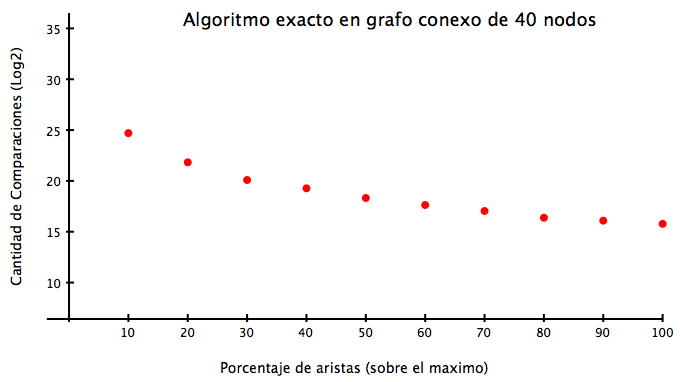
\includegraphics[scale=0.50]{Graficos/03-02.png}
\end{center}

Lo que podemos observar, como era de esperar, que cuantas menos aristas tenga el grafo m\'as comparaciones y peor se va a comportar el algoritmo. Esto se debe a que en un grafo muy denso los posibles subconjuntos independientes son menos que en el caso en el que tenga pocas aristas. Por esta razon en un grafo muy denso no se recorren muchas vecindades, lo que disminuye la cantidad de comparaciones. \\

\newpage

Por otro lado, mostramos a continuaci\'on el comportamiento del algoritmo, pero modificando la cantidad de nodos y su relaci\'on con las comparaciones que realiza el algoritmo exacto. \\
A medida que incrementamos la cantidad de nodos en los grafos, esperamos que la cantidad de comparaciones que realiza se incremente tambi\'en.

\begin{center}
	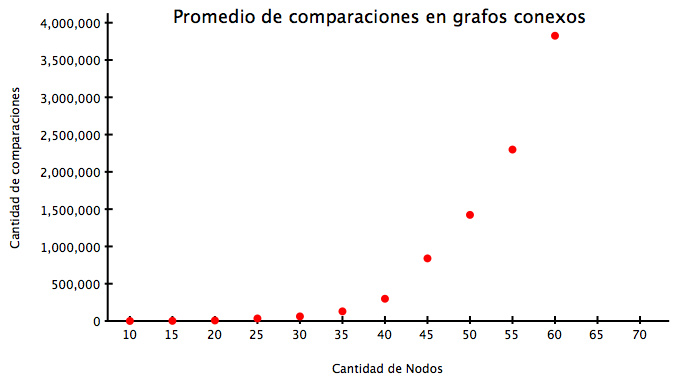
\includegraphics[scale=0.50]{Graficos/03-03.png}
\end{center}

Efectivamente, podemos ver que la cantidad de comparaciones que realiza el algoritmo seg\'un la cantidad de nodos, crece exponencialmente, como la complejidad del algoritmo. \\

Lo que realmente vemos en el gr\'afico es un promedio entre los valores obtenidos para los grafos evaluados.\\ 
Esta prueba se llevo a cabo sobre 50 grafos, de densidad variable entre el 30\% y el 60\% de las aristas y con pesos bien distribuidos.
Los grafos parten con 10 nodos, y se le incrementan de a 5 llegando hasta grafos de 120 nodos.
Estos ultimos no se muestran en el gr\'afico pues la cantidad de comparaciones era tan grande que hac\'ia despreciable la diferencia entre grafos con menos nodos.\\ 

\newpage

\section{Heur\'istica Constructiva}
\begin{itemize}
	\item Desarrollar e implementar una heur\'istica constructiva para CIMP.
\end{itemize}

\subsection{Descripci\'on de la Heur\'istica}
Una vez que leemos el archivo de entrada y tenemos todas las estructuras cargadas -la lista de adyacencia, los v\'ertices con sus atributos y la lista con los v\'ertices para recorrer, ordenados por peso de mayor a menor- comenzamos la ejecuci\'on de nuestra heur\'istica.\\

Para desarrollar la heur\'istica constructiva implementamos un algoritmo goloso, que partiendo de una lista de v\'ertices ordenada descendentemente por su peso, arma la soluci\'on eligiendo, en cada iteraci\'on, el primer v\'ertice que tenga disponible. \\

Para generar la soluci\'on, creamos un iterador para la lista de los v\'ertices del grafo, tomamos el primero y lo agregamos a la soluci\'on, esto lo podemos hacer ya que al ser el primer v\'ertice de la lista, no tiene ning\'un vecino que ya est\'e agregado. Al agregarlo, marcamos este v\'ertice como utilizado, e incrementamos en el contador de adyacencias a todos sus vecinos para que no se puedan agregar en las pr\'oximas iteraciones.\\

En la pr\'oxima iteraci\'on agregamos el siguiente v\'ertice que no est\'e marcado, es decir, que no tenga ning\'un vecino en la soluci\'on e incrementamos a los nodos adyacentes indicando que tienen un vecino m\'as que forma parte de la soluci\'on.\\

Continuamos iterando hasta que hayamos recorrido todos los v\'ertices que forman parte del grafo, agregando a la soluci\'on aqu\'ellos que no tengan vecinos ya agregados. \\

Veamos que el conjunto de v\'ertices que devuelve la heur\'istica constructiva es un conjunto independiente. Nosotros tenemos una lista de v\'ertices ordenada descendentemente por peso, e inicialmente agregamos a la soluci\'on el primer v\'ertice de la lista, y marcamos a sus vecinos para que no puedan ser agregados luego. En las pr\'oximas iteraciones, la heur\'istica va a recorrer los siguientes v\'ertices hasta encontrar alguno que no est\'e marcado, es decir, que no tenga ning\'un vecino que ya forme parte de la soluci\'on; y al agregarlo, incrementa en 1 el valor correspondiente de cada uno de sus adyacentes en el array \texttt{adyacencias}, para indicar que tienen un vecino m\'as en la soluci\'on. Seguimos ejecutando la heur\'istica de esta manera, hasta que hayamos recorrido todos los v\'ertices del grafo. Como la condici\'on para agregar un v\'ertice a la soluci\'on es que no tenga ning\'un vecino en ella, y al agregarlo marcamos a todos sus vecinos, sin obviar a ninguno, nunca vamos a tener dos nodos adyacentes en la soluci\'on, por lo tanto, el conjunto de v\'ertices que devuelve la heur\'istica constructiva es independiente.

\newpage

\subsection{Pseudoc\'odigo}
heuristicaConstructiva($Grafo \ G$) $\rightarrow$ Solucion. Genera una soluci\'on agregando nodos de mayor a menor (por peso) s\'olo si el nodo por agregar no es adyacente a ninguno que ya forme parte de la soluci\'on. \\

\begin{tabular}{rp{17cm}}
1: & 				heuristicaConstructiva($Grafo \ G$) \{\\
2: & \hspace{0,5cm} 	\paratodo (Vertice $vertice$ $\in$ vertices) \hacer \\
3: & \hspace{1cm} 		\iif ($vertice \ no \ tiene \ vecinos \ en \ solucion$)\\
4: & \hspace{1,5cm} 			agregarASolucion($vertice$)\\
5: & \hspace{1cm} 		\finif\\
6: & \hspace{0,5cm} 	\fin \\		
7: & \hspace{0,5cm}	\devolver $solucion$ \\	
8: & 				\}\\ \\
\end{tabular}

agregarASolucion ($Vertice v$). Agrega el v\'ertice $v$ a la soluci\'on que estamos generando, adem\'as, actualiza el peso de la misma, se marca ese v\'ertice como utilizado, y se incrementa la cantidad de vecinos en la soluci\'on de todos sus adyacentes. \\

\begin{tabular}{rp{17cm}}
1: & 				agregarASolucion($Vertice \ v$) \{\\
2: & \hspace{0,5cm} 	$agregar \ v \ al \ conjunto \ de \ vertices \ de \ la \ solucion$ \\
3: & \hspace{0,5cm} 	$sumar \ peso \ de \ v \ a \ la \ solucion$ \\
4: & \hspace{0,5cm} 	$marcar \ a \ v \ como \ usado$ \\
5: & \hspace{0,5cm} 	$deshabilitar \ vecinos \ de \ v \ para \ la \ solucion$ \\
6: & 				\}\\ \\
\end{tabular}

\subsection{C\'alculo de Complejidad}

\begin{itemize}
	\item Ordenar los nodos por peso y de forma descendente con un algoritmo Quicksort, es del orden de \ode{n^2}
	\item Verificar si se puede agregar un nodo a la soluci\'on toma \ode{1} pues es verificar que el contador de adyacencias de ese nodo este en 0.
	\item Agregar un nodo a la soluci\'on pertenece al orden \ode{d(v_i)} ya que tiene que incrementar el contador de adyacencias de sus vecinos.
	\item Para cada nodo que se puede agregar a la soluci\'on, lo agregamos.  \ode{d(v_i)}
\end{itemize}

\begin{center}
	\ensuremath{n^2 + \zum{i=1}{n}{d(v_i)} \leq n^2 + 2m \entonces \ode{n^2 + 2m} \pertenece \ode{n^2 + m}}
\end{center}

\underline{C\'alculo de Complejidad en funci\'on de la entrada}

\begin{center}
	\ensuremath{ T = log\ n + \zum{i=1}{n}{log\ p + \zum{j=1}{d(v_i)}{log\ v_j}} \mai log\ n + \zum{i=1}{n}{(log\ p + d(v_i))} \mai } \\
	\ensuremath{ log\ n + \zum{i=1}{n}{1} + \zum{i=1}{n}{d(v_i)} \mai log\ n + n + 2m} \\
	\vspace{1.5em}	
	\ensuremath{ \entonces T \mai n \ \wedge \ T \mai 2m \entonces T \mai m} \\
\end{center}

Como el algoritmo es \ode{n^2 + m} y $T \mai n \ \wedge \ T \mai m$ \entonces el algoritmo es \ode{T^2 + T} \pertenece \ode{T^2}

\newpage

­\subsection{Casos de Prueba y Gr\'aficos}

Debido que la complejidad de la heur\'istica es polinomial y no tiene sentido comparar la velocidad de esta heur\'istica con el algoritmo exacto, decidimos comparar la calidad de los resultados que arroja la heur\'istica frente a los obtenidos por el algoritmo exacto, para ver que tan ``bueno" \ es nuestro algoritmo goloso. \\

Para realizar estas pruebas generamos grafos al azar para evaluar los comportamientos en grafos generados de manera aleatoria, y ver que sin necesidad que cumplan alg\'un patr\'on los resultados de la heur\'istica son generalmente buenos. Armamos distintos casos de prueba que describiremos a continuaci\'on y compararemos los resultados obtenidos por la heur\'istica con los obtenidos por el algoritmo exacto, adem\'as, de esta forma podremos ver qu\'e tan buena es la soluci\'on con la que partiremos al ejecutar las heur\'isticas HBL y GRASP. Para hacer las pruebas, desarrollamos un algoritmo que genera grafos conexos, partiendo de un \'arbol y agregando aristas hasta la alcanzar la densidad buscada. Los pesos de estos grafos se generan aleatoriamente, acotados superior e inferiormente por un par\'ametro. \\

Dividimos los gr\'aficos de los casos de prueba seg\'un la densidad del grafo y la amplitud de los pesos. Observamos que cuando el grafo es menos denso, la calidad de la soluci\'on es mejor comparada a los otros casos. Esto se debe a que, como los v\'ertices no tienen tantos vecinos, cada vez que agregamos el nodo de mayor peso entre los disponibles, son menos los que anulamos para agregar a la soluci\'on en las pr\'oximas iteraciones. \\

\vspace*{2em}
\begin{center}
	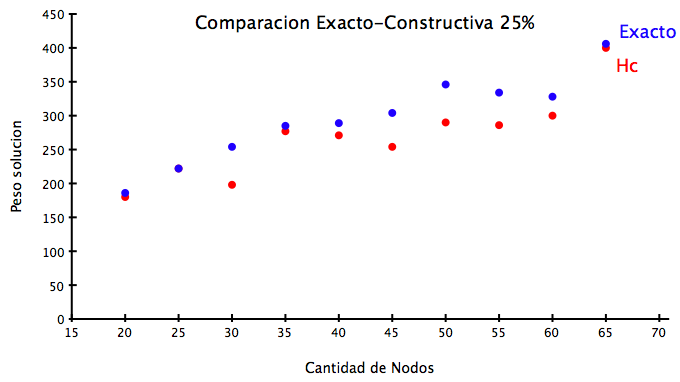
\includegraphics[scale=0.35,angle=00]{Graficos/04-02.png}
	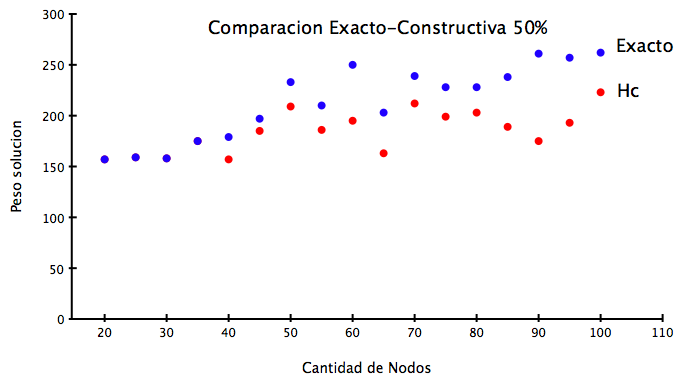
\includegraphics[scale=0.35,angle=00]{Graficos/04-03.png}
\end{center}

\vspace*{2em}

\begin{center}
	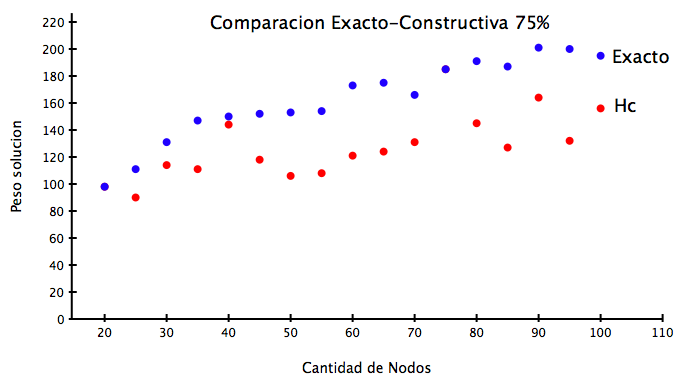
\includegraphics[scale=0.35,angle=00]{Graficos/04-04.png}
\end{center}

%\begin{center}
%	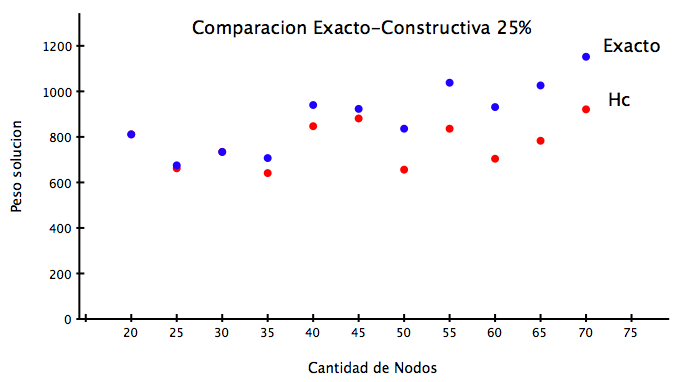
\includegraphics[scale=0.30,angle=90]{Graficos/04-05.png}
%	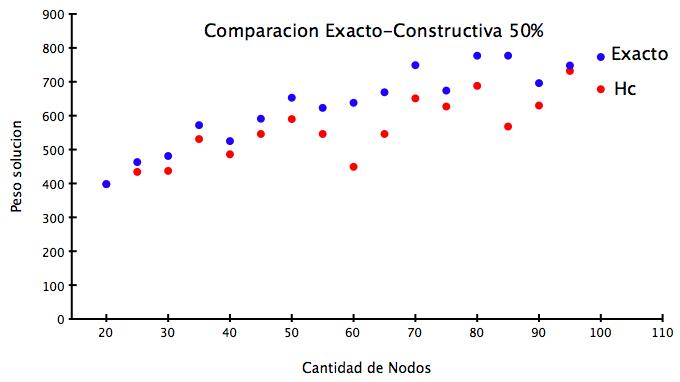
\includegraphics[scale=0.30,angle=90]{Graficos/04-06.png}
%	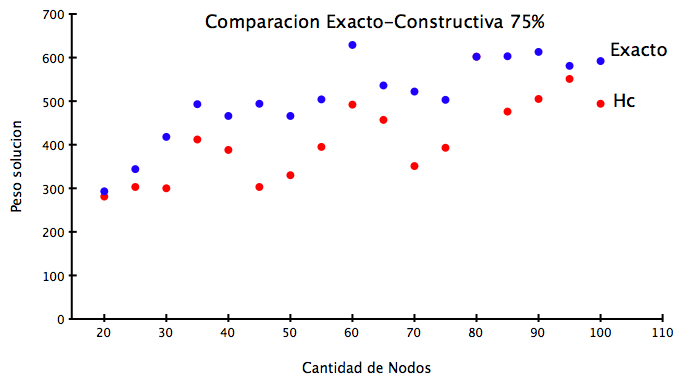
\includegraphics[scale=0.30,angle=90]{Graficos/04-07.png}
%\end{center}

%\begin{center}
%	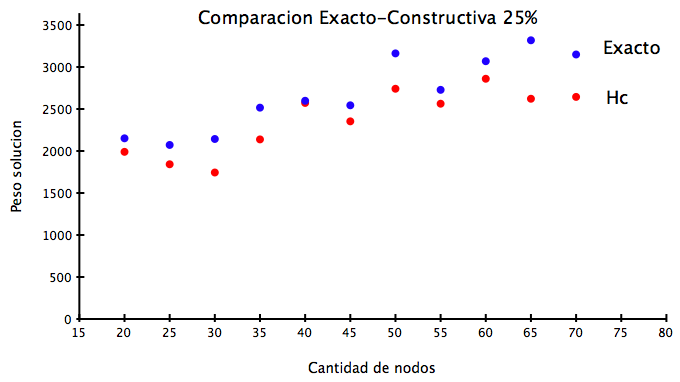
\includegraphics[scale=0.30,angle=90]{Graficos/04-08.png}
%	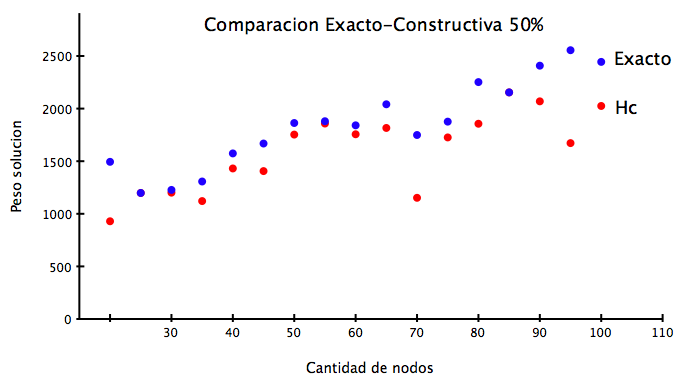
\includegraphics[scale=0.30,angle=90]{Graficos/04-09.png}
%	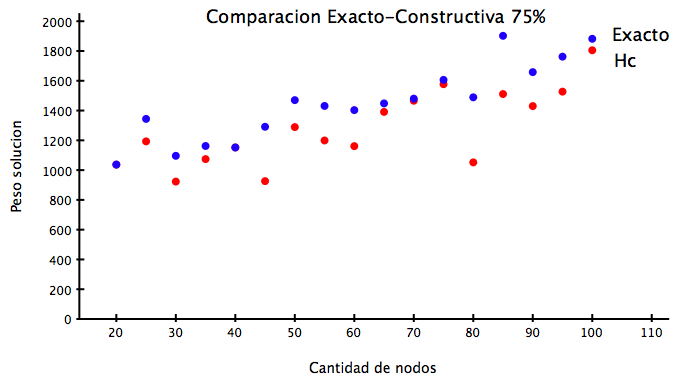
\includegraphics[scale=0.30,angle=90]{Graficos/04-10.png}
%\end{center}

\newpage

Haciendo los casos de prueba, pensamos en si la amplitud de los pesos de los nodos podr\'ia afectar la soluci\'on generada por la heur\'istica constructiva, ya que si tenemos un grafo en donde los pesos de los nodos no var\'ian mucho, nos podr\'ia pasar que agregamos a la soluci\'on el nodo disponible de mayor peso cuyos vecinos disponibles tienen peso menor, pero parecido al de \'este. Si podemos armar un conjunto independiente con estos nodos, como su peso no es mucho menor al del nodo elegido, el peso del conjunto podr\'ia superar notablemente al peso del nodo. Y en un grafo en donde la diferencia entre el peso m\'inimo y el peso m\'aximo es grande, la posibilidad de que ocurra esto es menor. \\

\begin{center}
	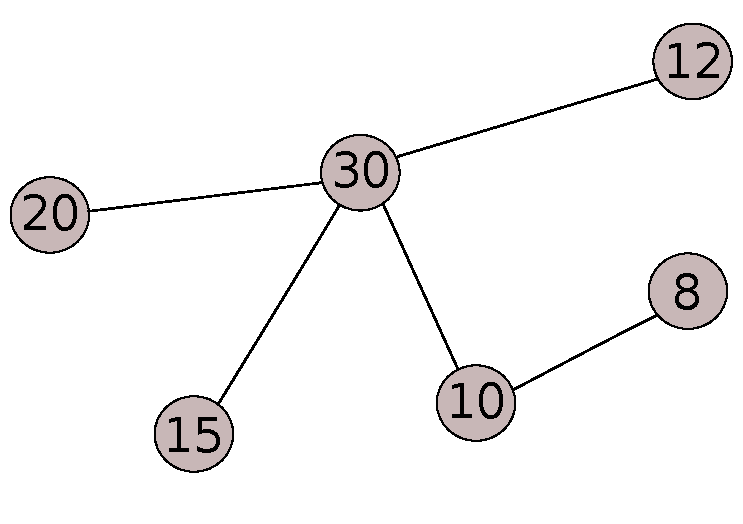
\includegraphics[scale=0.50]{Graficos/grafo.pdf}
\end{center}

La figura anterior ilustra lo que queremos evaluar. La heur\'istica agregar\'ia a la soluci\'on el nodo de peso 30, deshabilitando a sus vecinos para que puedan ser agregados luego. Sin embargo, podemos formar un conjunto independiente con estos nodos y su peso ser\'ia 57, que es bastante mayor. \\

Probamos con varios grafos conexos, y para obtener un resultado que sea v\'alido con respecto a lo que quer\'iamos testear, para cada uno de ellos mantuvimos la cantidad de nodos y la vecindad de cada uno de ellos, modificando s\'olo el rango del peso de cada nodo. Ejecutamos la heur\'istica constructiva y el algoritmo exacto para cada uno de estos grafos y obtuvimos los resultados que se ven reflejados en la siguiente tabla. \\

\begin{center}
\begin{tabular}{|c|c|c|c|c|c|}
\hline
\multicolumn{3}{|c|}{Grafos con Pesos de 10 a 300} & \multicolumn{3}{|c|}{Grafos con Pesos de 10 a 30} \\
\hline
Algoritmo & Heuristica & \multirow{2}{*}{Porcentaje} & Algoritmo & Heuristica & \multirow{2}{*}{Porcentaje} \\
Exacto & Constructiva & & Exacto & Constructiva & \\		
\hline
2024 & 1641 & 81.08\% & 238 & 165 & 69.33\% \\
2040 & 1711 & \textcolor{red}{83.87\%} & 237 & 207 & \textcolor{red}{87.34\%} \\
2151 & 1970 & 91.59\% & 241 & 196 & 81.33\% \\
2199 & 295 & \textcolor{red}{13.42\%} & 208 & 190 & \textcolor{red}{91.35\%} \\
2318 & 1727 & \textcolor{red}{74.5\%} & 222 & 217 & \textcolor{red}{97.75\%} \\
1964 & 1933 & 98.42\% & 242 & 204 & 84.3\% \\
2283 & 1786 & \textcolor{red}{78.23\%} & 243 & 203 & \textcolor{red}{83.54\%} \\
2397 & 1888 & 78.77\% & 236 & 167 & 70.76\% \\
2243 & 1888 & 84.17\% & 253 & 197 & 77.87\% \\
2185 & 1679 & \textcolor{red}{76.84\%} & 228 & 218 & \textcolor{red}{95.61\%} \\
2506 & 1799 & \textcolor{red}{71.79\%} & 236 & 188 & \textcolor{red}{79.66\%} \\
2153 & 1673 & \textcolor{red}{77.71\%} & 270 & 222 & \textcolor{red}{82.22\%} \\
1929 & 1380 & \textcolor{red}{71.54\%} & 225 & 166 & \textcolor{red}{73.78\%} \\
2108 & 1986 & 94.21\% & 226 & 162 & 71.68\% \\
2441 & 1955 & 80.09\% & 260 & 174 & 66.92\% \\
2494 & 1931 & 77.43\% & 247 & 165 & 66.8\% \\
2099 & 1683 & \textcolor{red}{80.18\%} & 226 & 209 & \textcolor{red}{92.48\%} \\
2326 & 2016 & 86.67\% & 242 & 160 & 66.12\% \\
2103 & 1629 & \textcolor{red}{77.46\%} & 242 & 199 & \textcolor{red}{82.23\%} \\
2265 & 1522 & \textcolor{red}{67.2\%} & 228 & 157 & \textcolor{red}{68.86\%} \\
\hline
\multicolumn{2}{|l|}{Promedio} & \textcolor{blue}{77.26\%} & \multicolumn{2}{|l|}{Promedio} & \textcolor{blue}{79.5\%} \\
\hline
\end{tabular}
\\
\end{center}

\newpage

Estos grafos est\'an formados por 80 nodos con una densidad del 50\%, cuyos pesos var\'ian como figura en la tabla. En cada l\'inea tenemos dos grafos isomorfos, cuya \'unica diferencia entre s\'i son los pesos. Podemos ver que en algunos casos el porcentaje del peso obtenido por la heur\'istica constructiva con respecto al del peso de la obtenida por el algoritmo exacto es mayor en los grafos con pesos m\'as grandes que en los grafos con pesos m\'as chicos, pero en otros casos es al rev\'es (los que escribimos en rojo). No s\'olo que no pudimos encontrar ning\'un patr\'on, sino que adem\'as al sacar el promedio de los promedios de cada tipo de grafos, la diferencia entre estos dos es despreciable. \\

Realizamos la misma prueba con distintos grafos, variando las densidades y todos con hasta 100 nodos (para poder ejecutar el algoritmo exacto) y en todos los casos la diferencia era despreciable, como en el caso que presentamos en esta tabla. Por lo tanto, la soluci\'on de la heur\'istica no es mejor ni peor dependiendo del intervalo que determina el peso de los nodos. \\

\subsection{Casos en los que el m\'etodo no proporciona una soluci\'on \'optima}

\begin{center}
	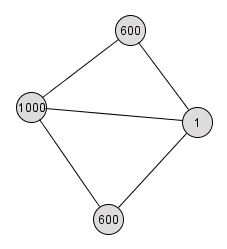
\includegraphics[scale=0.50]{Graficos/diamante.jpg}
\end{center}

Como podemos observar en este grafo, la heur\'istica constructiva nos devolver\'ia una soluci\'on formada por el nodo con peso 1000; y sin embargo, la soluci\'on \'optima est\'a formada por los dos nodos de peso 600. Esto ocurre debido a que la heur\'istica agrega a la soluci\'on los nodos de mayor peso siempre que no sea adyacente a ninguno de la soluci\'on. Esto queda salvado en $GRASP$ y la $busquedaLocal$.

Pero en la pr\'actica pudimos ver que no ocurre frecuentemente, y en B\'usqueda Local y GRASP queda salvado. En HBL, en alguna de las combinaciones, el nodo de 1000 ser\'ia quitado de la soluci\'on, pudi\'endose agregar los dos de 600 al buscar el mejor conjunto, y superando as\'i el peso de la soluci\'on anterior. Y en GRASP, con el factor aleatorio, puede ser que en alguna iteraci\'on se elija al de 1000, pero en otras, si los nodos adyacentes son bastante cercanos en cuanto al peso, puede tomarlos como inicio de la soluci\'on. Si no los toma por no entrar dentro del 20\% (como ser\'ia este caso), con B\'usqueda Local se solucionar\'ia este problema.
Esto es un problema que puede presentarse en la Heur\'istica Constructiva, pero que no afecta a la hora de tomarlo como par\'ametro para Hbl o GRASP, ya que cada uno a su manera lo puede solucionar.

\newpage

\section{Heur\'istica Busqueda Local}
\begin{itemize}
	\item Desarrollar e implementar una heur\'istica de busqueda local para CIMP.
\end{itemize}

\subsection{Descripci\'on de la Heur\'istica}
\subsubsection{Criterio de Vecindad}
Para hacer la b\'usqueda local primero tuvimos que decidir qu\'e criterio de vecindad tom\'abamos. En un primer momento pensamos en sacarle a la soluci\'on un porcentaje de nodos y luego agregar (como la heur\'istica constructiva) los posibles nodos. Pero luego en la pr\'actica, nos dimos cuenta que esto no aportaba mucho y que la vecindad era demasiado grande. \\

Impulsados por esto y luego de varias consultas, nos enfocamos en cambiar el criterio de vecindad. Primero, lo que decidimos fue no sacar un porcentaje de nodos, sino sacar un n\'umero fijo de la soluci\'on. Despues de hacer varias pruebas, conclu\'imos en sacar de la soluci\'on un subconjunto formado por 2 nodos, actualizando el conjunto de posibles v\'ertices para agregar a la soluci\'on. \\

Adem\'as modificamos la forma en que agregamos los nuevos posibles nodos que se habilitaron al sacar los 2 nodos de la soluci\'on. En vez de continuar con la heur\'istica constructiva decidimos encontrar el mejor conjunto (de 1, 2 o 3 elementos) independiente perteneciente a los posibles. La raz\'on por la cual fijamos de esa manera el cardinal del conjunto a agregar, es que luego de varios testeos, fue con el que obten\'iamos la mejor relaci\'on costo/beneficio. Luego s\'i, con el mismo criterio que la heur\'istica constructiva, le agregamos (si es que hay) los nodos que falten para hacer la soluci\'on maximal, cuidando que siga siendo independiente.

Aunque generar todos los conjuntos de 1, 2, o 3 elementos, y quedarnos con el que mejor incrementaba el peso de la soluci\'on, nos aumentaba la complejidad te\'orica, en la pr\'actica nos mejoraba much\'isimo la soluci\'on obtenida con un aumento despreciable del tiempo de ejecuci\'on.

\subsubsection{Explicaci\'on}
Sea $S$ la soluci\'on de un grafo conexo que recibe \'esta heur\'istica, calculamos las soluciones vecinas con el criterio de vecindad. \\

En esta etapa ten\'iamos dos opciones:

\begin{itemize}
	\item  $HBL1$: Movernos a la mejor soluci\'on vecina de todas las que mejoran, y partir de esta nueva soluci\'on.
	\item  $HBL2$: Movernos a la primer soluci\'on vecina que mejore y partir de esta nueva soluci\'on.
\end{itemize}

\begin{center}
\begin{tabular}{cc}
\begin{tabular}{|c|c|}
\hline
\multicolumn{2}{|c|}{HBL1} \\
\hline
Peso & Comparaciones \\
\hline
1547 & 2649214 \\
\hline
1602 & 1597778 \\
\hline
1646 & 2994873 \\
\hline
1723 & 3021388 \\
\hline
1337 & 3525897 \\
\hline
1690 & 1482242 \\
\hline
1944 & 1986955 \\
\hline
1911 & 1911242 \\
\hline
1771 & 1844278 \\
\hline
1814 & 1503834 \\
\hline
\end{tabular}
&
\begin{tabular}{|c|c|}
\hline
\multicolumn{2}{|c|}{HBL2} \\
\hline
Peso & Comparaciones \\
\hline
1516 & 2268464 \\
\hline
1602 & 1598084 \\
\hline
1640 & 2817863 \\
\hline
1744 & 2708938 \\
\hline
1312 & 2458041 \\
\hline
1690 & 1482548 \\
\hline
1944 & 1698988 \\
\hline
1911 & 1776960 \\
\hline
1771 & 1543561 \\
\hline
1814 & 1504254 \\
\hline
\end{tabular}
\end{tabular}
\end{center}

Observando esta tabla, decidimos quedarnos con la opci\'on HBL1, que se queda con la mejor soluci\'on vecina de toda la vecindad, a pesar de que \'esta realice m\'as comparaciones, el aumento del tiempo de ejecuci\'on era despreciable como para descartar esta opci\'on. \\

Una vez elegido el m\'etodo, lo que hacemos es, dada una soluci\'on, nos movemos a la mejor soluci\'on vecina, y volvemos a aplicar b\'usqueda local con esta nueva soluci\'on. Este procedimiento finaliza cuando, de una determinada soluci\'on, ninguna vecindad mejora o bien cuando mejor\'o cierta cantidad de veces. \\

Este p\'arametro $BQL\_VECES$ lo fijamos luego en los casos de prueba. \\

Veamos que la heur\'istica es correcta, es decir, que la soluci\'on que devuelve es un conjunto independiente. Nosotros partimos de una soluci\'on generada por la heur\'istica constructiva, que como ya vimos, es un conjunto independiente. En cada iteraci\'on, hacemos lo siguiente para cada componente conexa: para cada subconjunto de dos nodos, lo sacamos de la soluci\'on que ya ten\'iamos, y marcamos como disponibles los v\'ertices correspondientes (aqu\'ellos que, al haber sacado el subconjunto, no tienen vecinos en la soluci\'on). Hasta este punto, seguimos teniendo un conjunto independiente, ya que s\'olo eliminamos nodos de la soluci\'on sin agregar ninguno, lo cual no provoca que el conjunto pueda dejar de ser independiente. \\

En el siguiente paso, para cada v\'ertice que tengamos disponible, calculamos los subconjuntos independientes de 1, 2 \'o 3 nodos que se encuentran disponibles y lo contengan. Nos quedamos con el que sume el mayor peso y lo agregamos a la soluci\'on, actualizando para cada nodo fuera de la soluci\'on la cantidad de adyacentes que tiene en ella. Como los nodos de este conjunto eran nodos que estaban disponibles, y no son adyacentes entre s\'i, el conjunto de nodos no deja de ser un conjunto independiente despu\'es de agregar los v\'ertices, y por lo tanto, la soluci\'on que tenemos hasta ahora es v\'alida. \\

Puede ocurrir que al haber sacado 2 nodos de la soluci\'on y agregar 1, 2 \'o 3 v\'ertices nuevos, queden otros v\'ertices que no se encuentren en ella y que est\'en disponibles para agregar; en este caso, procedemos como en la heur\'istica constructiva, agregando los de mayor peso, siempre y cuando la soluci\'on no deje de ser un conjunto independiente. Y como \'estos estaban disponibles, no ten\'ian ning\'un vecino en la soluci\'on, por lo tanto, el conjunto de nodos de la soluci\'on sigue siendo un conjunto independiente y ahora es maximal. \\

Repetimos estos pasos para cada componente conexa, y una cantidad fija de veces ($BQL\_VECES$), en donde en cada iteraci\'on se genera una nueva soluci\'on parcial (si es que mejora la que ten\'iamos antes) y como vimos reci\'en, esta nueva soluci\'on tambi\'en es un conjunto independiente. Luego que la heur\'istica iter\'o la cantidad necesaria de veces y ha intentado mejorar cada componente conexa, nos devuelve la nueva soluci\'on. Cada componente conexa puede haber sido modificada para mejorar la soluci\'on que ten\'iamos antes, y el conjunto de v\'ertices de cada una de ellas sigue siendo un conjunto independiente, por lo tanto al unir todas estas componentes conexas para formar la nueva soluci\'on, los nodos de \'esta tambi\'en formar\'an un conjunto indepeniente. 

\subsection{Pseudoc\'odigo}

\begin{tabular}{rp{17cm}}
1: & 				busquedaLocal($Solucion \ solucionInicial$) \{ \\
2: & \hspace{0,5cm} 	\paracada ($ComponenteConexa\ C\ de\ G$) \hacer $BQL\_VECES$\\
3: & \hspace{1cm}			\asignar{solucionParcial}{solucionInicial} \\
4: & \hspace{1cm} 		\paracada (Subconjunto $s$ de 2 elementos) \\
5: & \hspace{1,5cm} 			$sacar\ s\ de\ solucionParcial$ \\
6: & \hspace{1,5cm} 			\asignar{conj}{mejorConjuntoDePosibles} \\
7: & \hspace{1,5cm} 			agregar $conj$ a la solucionParcial \\
8: & \hspace{1,5cm} 			completar la $solucionParcial$ para que sea maximal\\
9: & \hspace{1,5cm} 			\iif ($mejora\ la\ solucion$)\\
10: & \hspace{2cm} 				\asignar{mejorSolucion}{solucionParcial}\\
11: & \hspace{1,5cm} 		\finif\\
12: & \hspace{1cm} 		\fin \paracada \\
13: & \hspace{1cm} 		\asignar{solucionInicial}{mejorSolucion} \\
14: & \hspace{0,5cm} \fin \paracada \\
15: & \hspace{0,5cm} \devolver{mejor} \\ 
16: & 				\}\\ \\
\end{tabular}

\begin{tabular}{rp{17cm}}
1: & 								mejorConjuntoDePosibles($solucion$) \{ \\
2: & \hspace{0,5cm} 	\paratodo (nodo disponible para agregar, que no tiene ningun adyacente en la solucion) \hacer \\
3: & \hspace{1cm} 		\asignar{conj1}{mejor \ conjunto \ de \ 1 \ nodo} \\
4: & \hspace{1cm} 		\asignar{conj2}{mejor \ conjunto \ de \ 2 \ nodos \ que \ no \ sean \ adyacentes \ entre \ si} \\
5: & \hspace{1cm} 		\asignar{conj3}{mejor \ conjunto \ de \ 3 \ nodos \ que \ no \ sean \ adyacentes \ entre \ si} \\
6: & \hspace{0,5cm} 	\fin \paratodo \\
7: & \hspace{0,5cm} 	\devolver{el mejor conjunto de los 3 (el mas pesado)} \\
8: & 			\}\\ \\
\end{tabular}

\subsection{C\'alculo de Complejidad}
Sea $n_c$ la cantidad de nodos de un grafo conexo y $m_c$ la cantidad de aristas del mismo.
Calculemos la complejidad para un grafo conexo:
\begin{itemize}
	\item Tomar todos los posibles conjuntos de 2 nodos para quitar de la soluci\'on. \ode{n_c^2}
	\item A cada conjunto formado de 2 nodos para quitar, lo quitamos de la soluci\'on, habilitando nodos posibles a agregar. \ode{n_c}
	\item Tomar el conjunto de mayor peso de los conjuntos posibles de 1, 2 y 3 elementos dentro de los nodos posibles a agregar pertenece al orden de 			\ode{n_c + n_c^2 + n_c^3} \entonces \ode{n_c^3}
	\item Agregar el mejor conjunto seleccionado anteriormente a la soluci\'on. \ode{d(v)} $\leq$ \ode{n_c}
	\item Completar la soluci\'on con los nodos posibles, hasta que sea maximal \ode{lon(posibles)} $\leq$ \ode{n_c}
\end{itemize}

\begin{center}
	\ensuremath{n_c^2 \times (n_c + n_c^3 + n_c + n_c) \entonces n_c^2 \times (n_c^3 + 3n_c) } \\ \vspace*{1em}
	\ensuremath{ \entonces \ode{n_c^2} \times \ode{n_c^3} \entonces \ode{n_c^5}}
\end{center}

Ahora, si consideramos que un grafo puede tener $ccc$ componentes conexas, el calculo final del algoritmo seria:
\begin{itemize}
	\item Separar en componentes conexas, utilizando BFS. \ode{n + m}
	\item A cada componente conexa, aplicar el algoritmo para grafos conexos antes descrito. \ode{n_c^5}
\end{itemize}

Pero, el peor caso lo encontramos cuando $ccc = 1$, o sea la cantidad de nodos de la \'unica componente conexa es $n$, pues la cantidad de subconjuntos ($2^n$) que se pueden formar es mayor, por lo tanto, habr\'ia m\'as soluciones que comprobar.

La complejidad es:

\begin{center}
	\ensuremath{n + m + \zum{i=1}{ccc}{n_c^5} \entonces n + m + \zum{i=1}{1}{n^5} \entonces n + m + n^5 \pertenece \ode{n+m+n^5} \pertenece \ode{n^5}} \\ 
\end{center}

\vspace*{2em}
\underline{C\'alculo de Complejidad en funci\'on de la entrada}

\begin{center}
	\ensuremath{ T = log\ n + \zum{i=1}{n}{log\ p + \zum{j=1}{d(v_i)}{log\ v_j}} \mai log\ n + \zum{i=1}{n}{(log\ p + d(v_i))} \mai } \\
	\ensuremath{ log\ n + \zum{i=1}{n}{1} + \zum{i=1}{n}{d(v_i)} \mai log\ n + n + 2m} \\
	\vspace{1em}	
	\ensuremath{ \entonces T \mai n} \\
\end{center}

Como el algoritmo es \ode{n^5} y $T \mai n$ \entonces el algoritmo es \ode{T^5}

\newpage

\subsection{Casos de Prueba y Gr\'aficos}

Para poder fijar la cantidad de vecindades a recorrer, debemos evaluar donde nuestra heur\'istica obtiene mejores resultados.
Para esta evaluaci\'on, creamos 1630 grafos conexos, entre 100 y 1000 nodos al azar, y con densidad variable de aristas.
Una vez que creamos los grafos, para cada uno utilizamos la Heur\'istica de Busqueda Local y guardamos la cantidad de vecindades que recorri\'o.
Forzosamente recorremos 400 vecindades, para asegurarnos que mejora lo m\'as posible.

Llevamos una suma de la cantidad de vecindades que recorri\'o en cada caso, y las agrupamos en peque\~nos intervalos, asi podemos observar cuantas vecindades deber\'iamos recorrer para asegurarnos un buen resultado de parte de la heur\'istica.

\begin{center}
	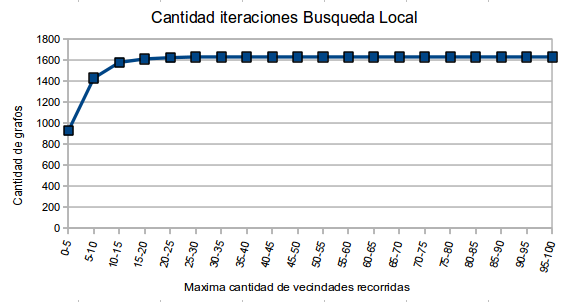
\includegraphics[scale=0.65]{Graficos/05-01.png}
\end{center}

Podemos ver que la pendiente de crecimiento de la curva, a medida que se incrementa la cantidad de vecindades recorridas, va disminuyendo hasta llegar a 0. \\
Esto significa que la busqueda local encontr\'o su vecino m\'aximo antes que llegue a 0 la pendiente.
En el gr\'afico vemos que esto sucede alrededor de las 30 vecindades recorridas, pero como la diferencia en tiempo de ejecuci\'on de recorrer 30 vecindades y 50 es despreciable, elegimos como par\'ametro, recorrer 50 vecindades para tener un espectro m\'as grande y mejorar algun otro grafo que todav\'ia puede mejorar. ($BQL\_VECES = 50$)

\newpage

\section{Metaheur\'istica GRASP}
\begin{itemize}
	\item Desarrollar e implementar una metaheur\'istica GRASP.
\end{itemize}

\subsection{Descripci\'on de la metaheur\'istica}
Una metaheur\'istica es una estrategia de alto nivel que utiliza otras heur\'isticas para alcanzar o mejorar una soluci\'on. En particular, una metaheur\'istica GRASP se compone en una heur\'istica constructiva para obtener una soluci\'on inicial, - aplic\'andole un factor de aleatoriedad para no generar siempre la misma soluci\'on inicial - y una heur\'istica de b\'usqueda local para mejorar la soluci\'on inicial. \\

En nuestro caso, aplicamos una heur\'istica constructiva como la antes descrita; s\'olo que, para ir formando la soluci\'on, tomamos aleatoriamente un nodo de un porcentaje de los nodos de mayor peso. Este $PORCENTAJE$ es un par\'ametro que luego fijaremos al final de los casos de prueba. \\

Veamos que esta soluci\'on es un conjunto independiente. Esta heur\'istica funciona igual que la heur\'istica constructiva, con la diferencia que en lugar de tomar el nodo de peso m\'aximo en cada iteraci\'on, tomamos uno al azar de los de mayor peso, o sea los que se encuentran dentro del par\'ametro $pocentaje$. Una vez que tenemos este nodo, queremos ver si podemos agregarlo a la soluci\'on, esto lo podemos hacer s\'olo si este nodo no tiene ning\'un vecino que ya se encuentre en ella, de ser as\'i, lo agregamos y actualizamos el estado de sus vecinos, indicando que tienen un adyacente m\'as en la soluci\'on. Procedemos de la misma forma, hasta no tener m\'as nodos disponibles para agregar. Cada vez que que agregamos un nodo a la soluci\'on verificamos que \'este no sea adyacente a ninguno que ya se encuentre en ella, y luego de agregarlo (si es posible) marcamos a todos sus vecinos indicando que tienen un vecino m\'as en la soluci\'on. Por lo tanto los nodos que figuran como disponibles son s\'olo aqu\'ellos que no tienen ning\'un adyacente en la soluci\'on parcial que estamos generando, y son los \'unicos que podr\'an ser agregados a la soluci\'on en futuras iteraciones. Luego, la soluci\'on que generamos es un conjunto independiente de nodos. \\

Luego de obtener la soluci\'on inicial, a \'esta le aplicamos la misma b\'usqueda local que definimos anteriormente y nos quedamos con la nueva soluci\'on si es de mejor peso. Como vimos anteriormente, la Heur\'istica de B\'usqueda Local puede modificar la soluci\'on, pero \'esta sigue siendo un conjunto independiente. Este procedimiento lo realizamos $CANTIDAD\_VECES$ veces, ya que como el resultado obtenido tiene un factor de aleatoriedad, no siempre va a ser la mejor soluci\'on. Es por esto que la ejecutamos varias veces y nos quedamos con la soluci\'on de mayor peso de todas las que obtuvimos. \\

Nuestra heur\'istica obtiene $CANTIDAD\_VECES$ soluciones, que son conjuntos independientes, y devuelve s\'olo aqu\'ella de mayor peso. Por lo tanto, la soluci\'on obtenida por la Heur\'istica GRASP tambi\'en es conjunto independiente de v\'ertices. \\

\newpage

\subsection{Pseudoc\'odigo}
metaheuristicaGRASP($Grafo\ G$) $\rightarrow$ Solucion. Devuelve la mejor soluci\'on encontrada, luego de $CANTIDAD\_VECES$ iteraciones. \\

\begin{tabular}{rp{17cm}}
1: & 				metaheuristicaGRASP($Grafo \ G$) \{\\
2: & \hspace{0,5cm} 	\repetir $CANTIDAD\_VECES$ \\
3: & \hspace{1cm} 		\asignar{solucionParcial}{heuristicaContructivaAleatoria($vertices$, PORCENTAJE)}\\
4: & \hspace{1cm} 		\asignar{solucionParcial}{busquedaLocal(solucionParcial)}\\
5: & \hspace{1cm} 		\iif ($es\ mejor\ que\ la\ solucion\ global$)\\
6: & \hspace{1,5cm} 			\asignar{solucionGlobal}{solucionParcial}\\
7: & \hspace{1cm} 		\finif\\
8: & \hspace{0,5cm} 	\fin \\		
9: & \hspace{0,5cm}	\devolver $solucionGlobal$ \\	
10: & \}\\ \\
\end{tabular}

heuristicaContructivaAleatoria() $\rightarrow$ Solucion. Devuelve la mejor soluci\'on encontrada, luego de $CANTIDAD\_VECES$ iteraciones. \\

\begin{tabular}{rp{17cm}}
1: & 				heuristicaContructivaAleatoria($vertices$, $PORCENTAJE$) \{\\
2: & \hspace{0,5cm} 	\mientras ($vertices$ no este vac\'io) \hacer \\
3: & \hspace{1cm} 		\asignar{v}{tomar\ uno\ al\ azar\ del\ $PORCENTAJE$\ de\ los\ mas\ grandes} \\
4: & \hspace{1cm} 		\iif ($v \ no \ tiene \ vecinos \ en \ solucion$)\\
5: & \hspace{1,5cm} 			agregarASolucion($v$)\\
6: & \hspace{1cm} 		\finif\\
7: & \hspace{1cm} 		sacarDeVertices($v$)\\
8: & \hspace{0,5cm} 	\fin \\		
9: & \hspace{0,5cm}	\devolver $solucion$ \\	
10: & 				\}\\ \\
\end{tabular}

\subsection{C\'alculo de Complejidad}

\begin{itemize}
	\item Generar una soluci\'on inicial aleatoria, partiendo de una heur\'istica constructiva. \ode{n^2+m}
	\item Aplicar busqueda local a esta soluci\'on. \ode{n^6}
	\item Actualizar la solucion. \ode{1}
	\item Repetir este proceso $CANTIDAD\_VECES$. \ode{k}
\end{itemize}

\begin{center}
	\ensuremath{ k \times (n^2 + m + n^6) \entonces \ode{k \times (n^2 + m + n^6)} \pertenece k \times \ode{n^6} \pertenece \ode{n^6}}
\end{center}

\newpage

\subsection{Casos de Prueba y Gr\'aficos}

Tenemos que decidir dos par\'ametros para nuestra Heur\'istica GRASP.

Para determinar la $CANTIDAD\_VECES$ que ejecutamos GRASP, utilizamos el mismo proceso que en Busqueda Local.
Acumulamos el n\'umero de iteraciones donde el algoritmo alcanzo el m\'aximo y lo volcamos en un gr\'afico.

A diferencia de la Busqueda Local, GRASP demora mucho m\'as tiempo, entonces redujimos la cantidad de grafos donde testear la heur\'istica.
Creamos 600 grafos, con alrededor de 100 y 1000 nodos, pero con una densidad media de aristas. 

\begin{center}
	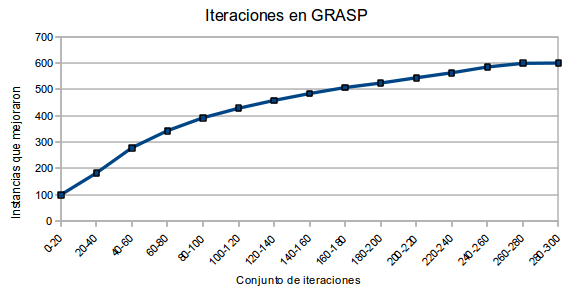
\includegraphics[scale=0.60]{Graficos/06-01.png}
\end{center}

Nuevamente, la pendiente de la curva nos informa donde el algoritmo llega a sus m\'aximos.
En este caso, la pendiente no se vuelve 0 tan rapidamente como en la Busqueda Local, pero si podemos ver una gran diferencia alrededor de las 120 iteraciones, que es donde cada vez menos grafos llegan a alcanzar el m\'aximo. \\
Pese a que la heur\'istica sigue mejorando con m\'as iteraciones, se vuelve un proceso muy costoso con respecto al tiempo de ejecuci\'on.
Por eso decidimos fijar el par\'ametro en 150, que es donde la pendiente va decreciendo, y en la mayor\'ia de los casos queda cubierta la mejor soluci\'on. ($CANTIDAD\_VECES = 150$) \\ 

Otro de los par\'ametros a tomar en cuenta para este algoritmo es el porcentaje de la lista restringida de candidatos (RCL) que se utiliza en el algoritmo constructivo. Para realizar estas pruebas, en cada gr\'afico tomamos 10 instancias de grafos conexos de 1000 nodos. Primero generamos los 10 grafos tal que tengan una baja densidad y corrimos la heur\'istica de GRASP para cada uno de ellos. \\

\begin{center}
	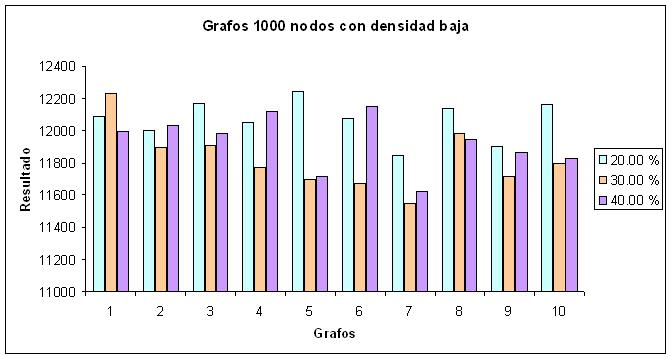
\includegraphics[scale=0.60]{Graficos/06-02.jpg}
\end{center}

\newpage

Para este segundo gr\'afico generamos nuevamente 10 instancias, pero esta vez cada instancia ten\'ia una densidad mayor al 75\%. \\

\begin{center}
	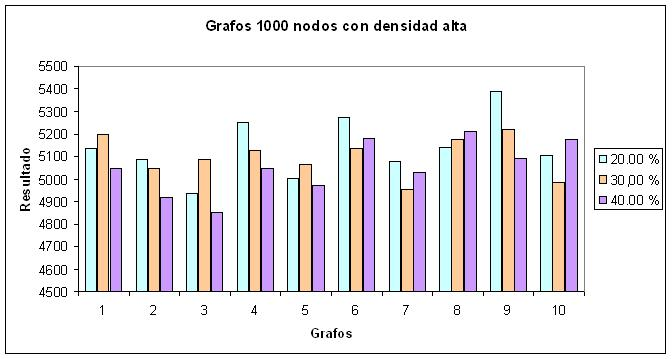
\includegraphics[scale=0.60]{Graficos/06-03.jpg}
\end{center}

En ambos gr\'aficos podemos ver que, si bien no ocurre en la totalidad de los casos, el resultado mayor se obtiene cuando el porcentaje de la RCL es del 20\%. \\ 

Este par\'ametro est\'a muy ligado al de la cantidad de iteraciones de GRASP, y a la cantidad de nodos del grafo. Dependiendo del tiempo disponible que tengamos para lograr una mejor relaci\'on tiempo-benficio, vemos que cuanto mayor sea el porcentaje de la RCL, mayor va a ser el n\'umero de diferentes resultados generados por el algoritmo constructivo, pero por tal motivo necesitar\'iamos m\'as iteraciones de GRASP, lo cual inevitablemente ser\'ia mucho m\'as costoso en tiempo. \\

Por esta raz\'on es la que decidimos fijar el par\'ametro del porcentaje de la RCL en 20\%, ya que es el que mejor resultados nos da, asumiendo que tenemos un tiempo acotado para conseguir la mejor relaci\'on tiempo-beneficio. Pero sin duda si tuviesemos algo m\'as de tiempo aumentar\'iamos este par\'ametro conjuntamente con el de iteraciones de GRASP. ($PORCENTAJE = 20$) \\

\newpage

\section{Conclusiones}

Luego de fijar los parametros de la heur\'istica GRASP, quisimos hacer un grafico final para comparar los resultados de las diferentes heur\'isticas.

Para comparar el comportamineto de las diferentes heur\'isticas, conjuntamente con GRASP lo que hicimos fue correr los tres algoritmos (HC, HBL, GRASP) sobre las mismas instancias. \\
Utilizamos diez instancias de pruebas con las siguientes caracteristicas.
\begin{itemize}
	\item Grafo conexo
	\item 500 nodos
	\item Incrementamos las aristas de a un 5\%
\end{itemize}

Utilizamos grafos de 500 nodos, ya que con la cantidad de instancias que iba a correr, demoraba mucho tiempo, pero el comportamiento que queriamos destacar, se puede observar de todas maneras.

\begin{center}
	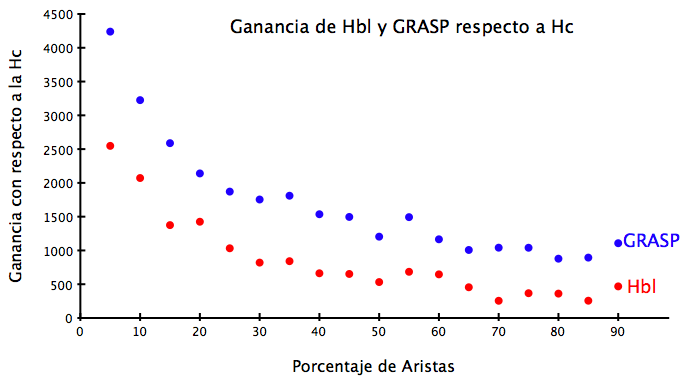
\includegraphics[scale=0.50]{Graficos/07-01.png}
\end{center}

En este gr\'afico queremos mostrar la diferencia de los resultados generados por $GRASP$ y $HBL$ con respecto al de la \textit{heur\'istica Constructiva}. Como podemos observar en el gr\'afico, en todos los casos $GRASP$ nos da un mejor resultado, como era de esperar. Sobre todo en los casos en los que $HBL$ cae en un m\'aximo local en la vecindad de la soluci\'on dada por la \textit{heur\'istica Constructiva}. \\

\section{Conclusion Final}
Como conclusi\'on de este trabajo destacamos la importancia de las heur\'isticas como recursos para resolver problemas en los cuales el algoritmo exacto es exponencial, con lo cual, no se podr\'ian resolver instancias con un tama\~no de entrada grande, ya que demandar\'ia incluso a\~nos de tiempo de ejecuci\'on. \\ 

Como vimos a lo largo de todo el trabajo, estas heur\'isticas nos permiten acercarnos a una buena soluci\'on en un tiempo razonable. \\
Por otra parte, si quisieramos mejores resultados podr\'iamos invertir tiempo de ejecuci\'on, lo que nos proporcionaria soluciones m\'as cercanas a la \'optima, pero eso depende de las necesidades de cada problema. \\


\end{document}